\chapter{Architecture}
% OR: \chapter{Model}
\label{cha:architecture}

\begin{comment}
Here you will present the architecture or model that you have chosen and which is (or will be) implemented in your work.
Note that putting algorithms in your report is not always desirable, so in certain cases those might be placed in the appendix.
Code is normally to be avoided in the report itself, but may be included in an appendix or submitted as additional documents.
(The actual code must also be submitted together with the final Master's thesis, but as a zip-file.)

Any off-the-shelf tools and methods that you use in your architecture should have been introduced earlier,
tentatively in the Background chapter (or in the Related Work chapter),
so that they can be referenced here by giving backward pointers to the previous text.

Here, or in a separate chapter (or possibly in the Background chapter or in the Experimental Setup),
you should also discuss the data that you use in your experiments (see Chapter~\ref{cha:data}).

\textit{Nunc in tristique risus, ut malesuada tortor. Integer ullamcorper nunc a felis vehicula condimentum. Aliquam eget turpis purus. Nam nec ipsum sed ligula vulputate tempor ac non arcu. Aenean hendrerit pretium ante et suscipit. Proin vitae venenatis ex, at pellentesque erat. Nulla facilisi. Sed quis eros lorem. Praesent id pharetra risus. Nunc a lacinia est. Nunc in urna at purus ullamcorper blandit eget sit amet est. Cras sagittis et ante ut lobortis. Proin quis arcu eros. Aliquam tempor neque vehicula lacus placerat, ac ultricies massa ultricies. Aliquam et nulla eget felis accumsan rutrum quis sed ligula.}

\textit{Vivamus bibendum tempus tincidunt. Integer imperdiet lectus pellentesque, rhoncus quam at, tempor ex. Phasellus semper tempor sapien at consequat. Proin ut dolor interdum, ullamcorper leo ac, convallis metus. Nullam tincidunt, metus ullamcorper sodales placerat, ipsum ipsum porttitor est, id volutpat orci orci sit amet quam. Vestibulum sagittis urna sit amet nulla vulputate, nec pellentesque enim hendrerit. Suspendisse at laoreet ipsum. Phasellus arcu nisi, laoreet sed tellus sit amet, imperdiet fringilla ante. Quisque rhoncus accumsan magna vel posuere. Fusce facilisis est eros, ac viverra diam maximus ut. Nullam ut lectus nunc. Fusce vestibulum sem at ex euismod tempus. Lorem ipsum dolor sit amet, consectetur adipiscing.}

\textit{Phasellus sed ipsum nunc. Nam iaculis felis mauris, sit amet condimentum ex malesuada at. Morbi lacinia odio mi, sit amet pellentesque ante facilisis sit amet. In lobortis elit ut dictum mollis. Aliquam erat volutpat. Morbi sit amet metus nisi. Nulla auctor varius metus at rhoncus. Pellentesque porta mollis leo, eu ultricies nulla mollis ac. Vivamus interdum ac odio vitae sodales. Aenean finibus eros rhoncus molestie elementum. Integer maximus erat vitae purus lobortis iaculis. Etiam blandit varius nulla, sed euismod felis.}

Clearly, a figure showing the architecture is a must, such as Figure~\ref{fig:Architecture}.
Describe all parts of such a figure in reasonable detail in the text, possibly with forward pointers to sections where they will be elaborated on (or backward pointers to sections where tools and methods already have been introduced).
Mention work that motivated your architectural choices, parameter settings, etc.
Those choices should then also be discussed and elaborated on in the Discussion chapter.

\begin{figure}[t!]
    \centering
    \missingfigure{Architecture figure to be added}
    \caption{The missing architecture}
    \label{fig:Architecture}
\end{figure}
\end{comment}

\section{High-Level Application Architecture}

A microservice architecture was employed in order to simplify development and separate concerns between the different microservices. The services are deployed as Docker Containers, and they are orchestrated using Docker Compose. \todo{quickly explain docker and why it is useful here} \autoref{fig:architecture-overview} shows how the application is divided into five distinct services, and the direction of information flow between these.

\begin{figure}[h]
    \centering
    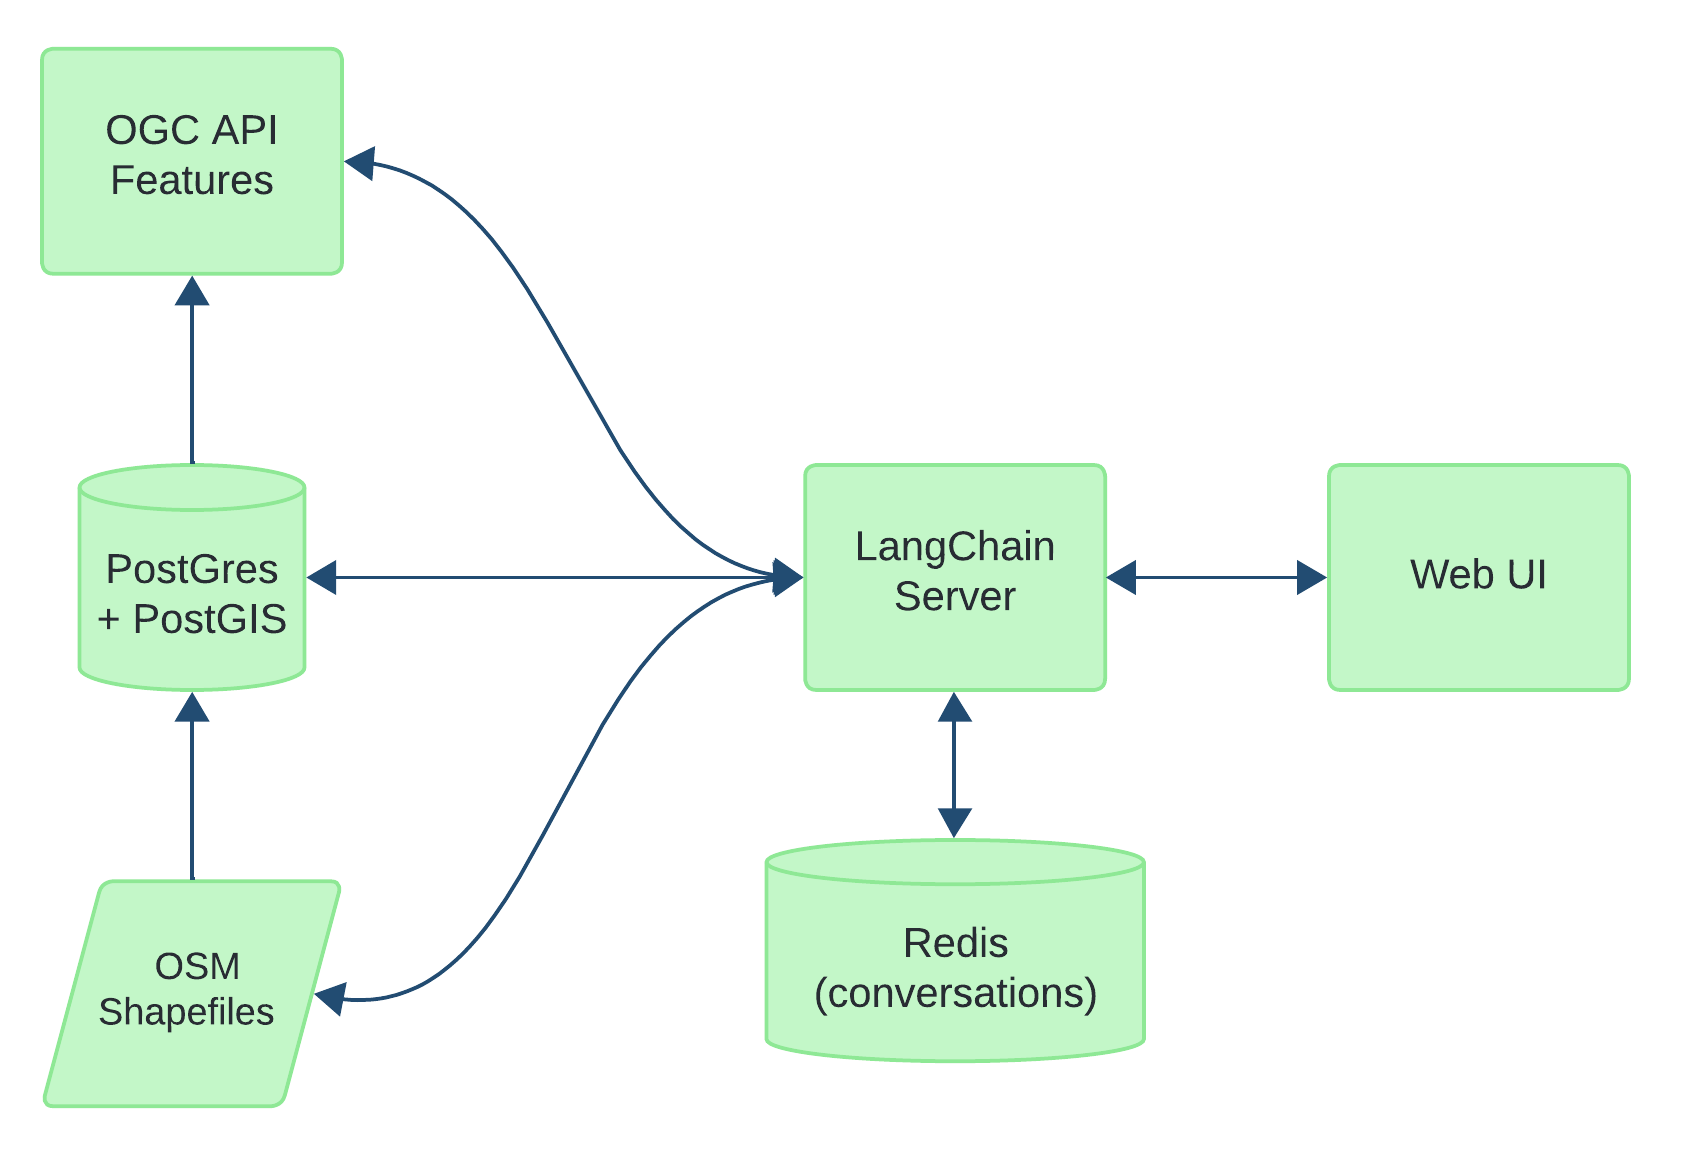
\includegraphics[width=\textwidth]{microservices.png}
    \caption{Architecture overview}
    \label{fig:architecture-overview}
\end{figure}



\subsection{LangChain Server}\label{subsec:langchain}

The \textit{LangChain Server} service is the heart of the application, and is where the \gls{acr:llm}-related logic is situated. It is responsible for taking requests from the \textit{Web \acrshort{acr:ui}} and returning suitable responses in what becomes a client-server architecture between the two services. \autoref{tbl:server-endpoints} show the endpoints exposed by the server and how they can be used by a client.

\begin{table}[h]
    \centering
    \caption{Summary of Server Endpoints}
    \label{tbl:server-endpoints}
    \begin{tabular}{p{0.22\textwidth}p{0.1\textwidth}p{0.55\textwidth}}
        \toprule
        \textbf{Endpoint} & \textbf{Method} & \textbf{Description}                                                                                                                                                         \\
        \midrule
        /session          & GET             & Takes a \texttt{session\_id} as a query parameter, allowing the client to continue on a pre-existing session.                                                                \\
        /session          & POST            & Creates a new session with an empty conversation.                                                                                                                            \\
        /streaming-chat   & GET             & Endpoint for chatting the \acrshort{acr:llm}. Takes a \texttt{message} as a query parameter and returns an event stream, allowing for token streaming from server to client. \\
        /update-map-state & POST            & Send the state of the client map to the server. Keeps the server updated on what layers are present in the map, their color, etc.                                            \\
        /geojson          & GET             & Takes a \texttt{geojson\_path} as a query parameter. Allows the client to retrieve a given GeoJSON file that is stored in the working directory on the server.               \\
        % /history          & GET             & Used to retrieve the chat history of the current session.                                                                                                                    \\
        /upload           & POST            & Allows the client to upload one or more files to the working directory on the server.                                                                                        \\
        \bottomrule
    \end{tabular}
\end{table}

\begin{figure}
    % \centering
    \makebox[\textwidth][c]{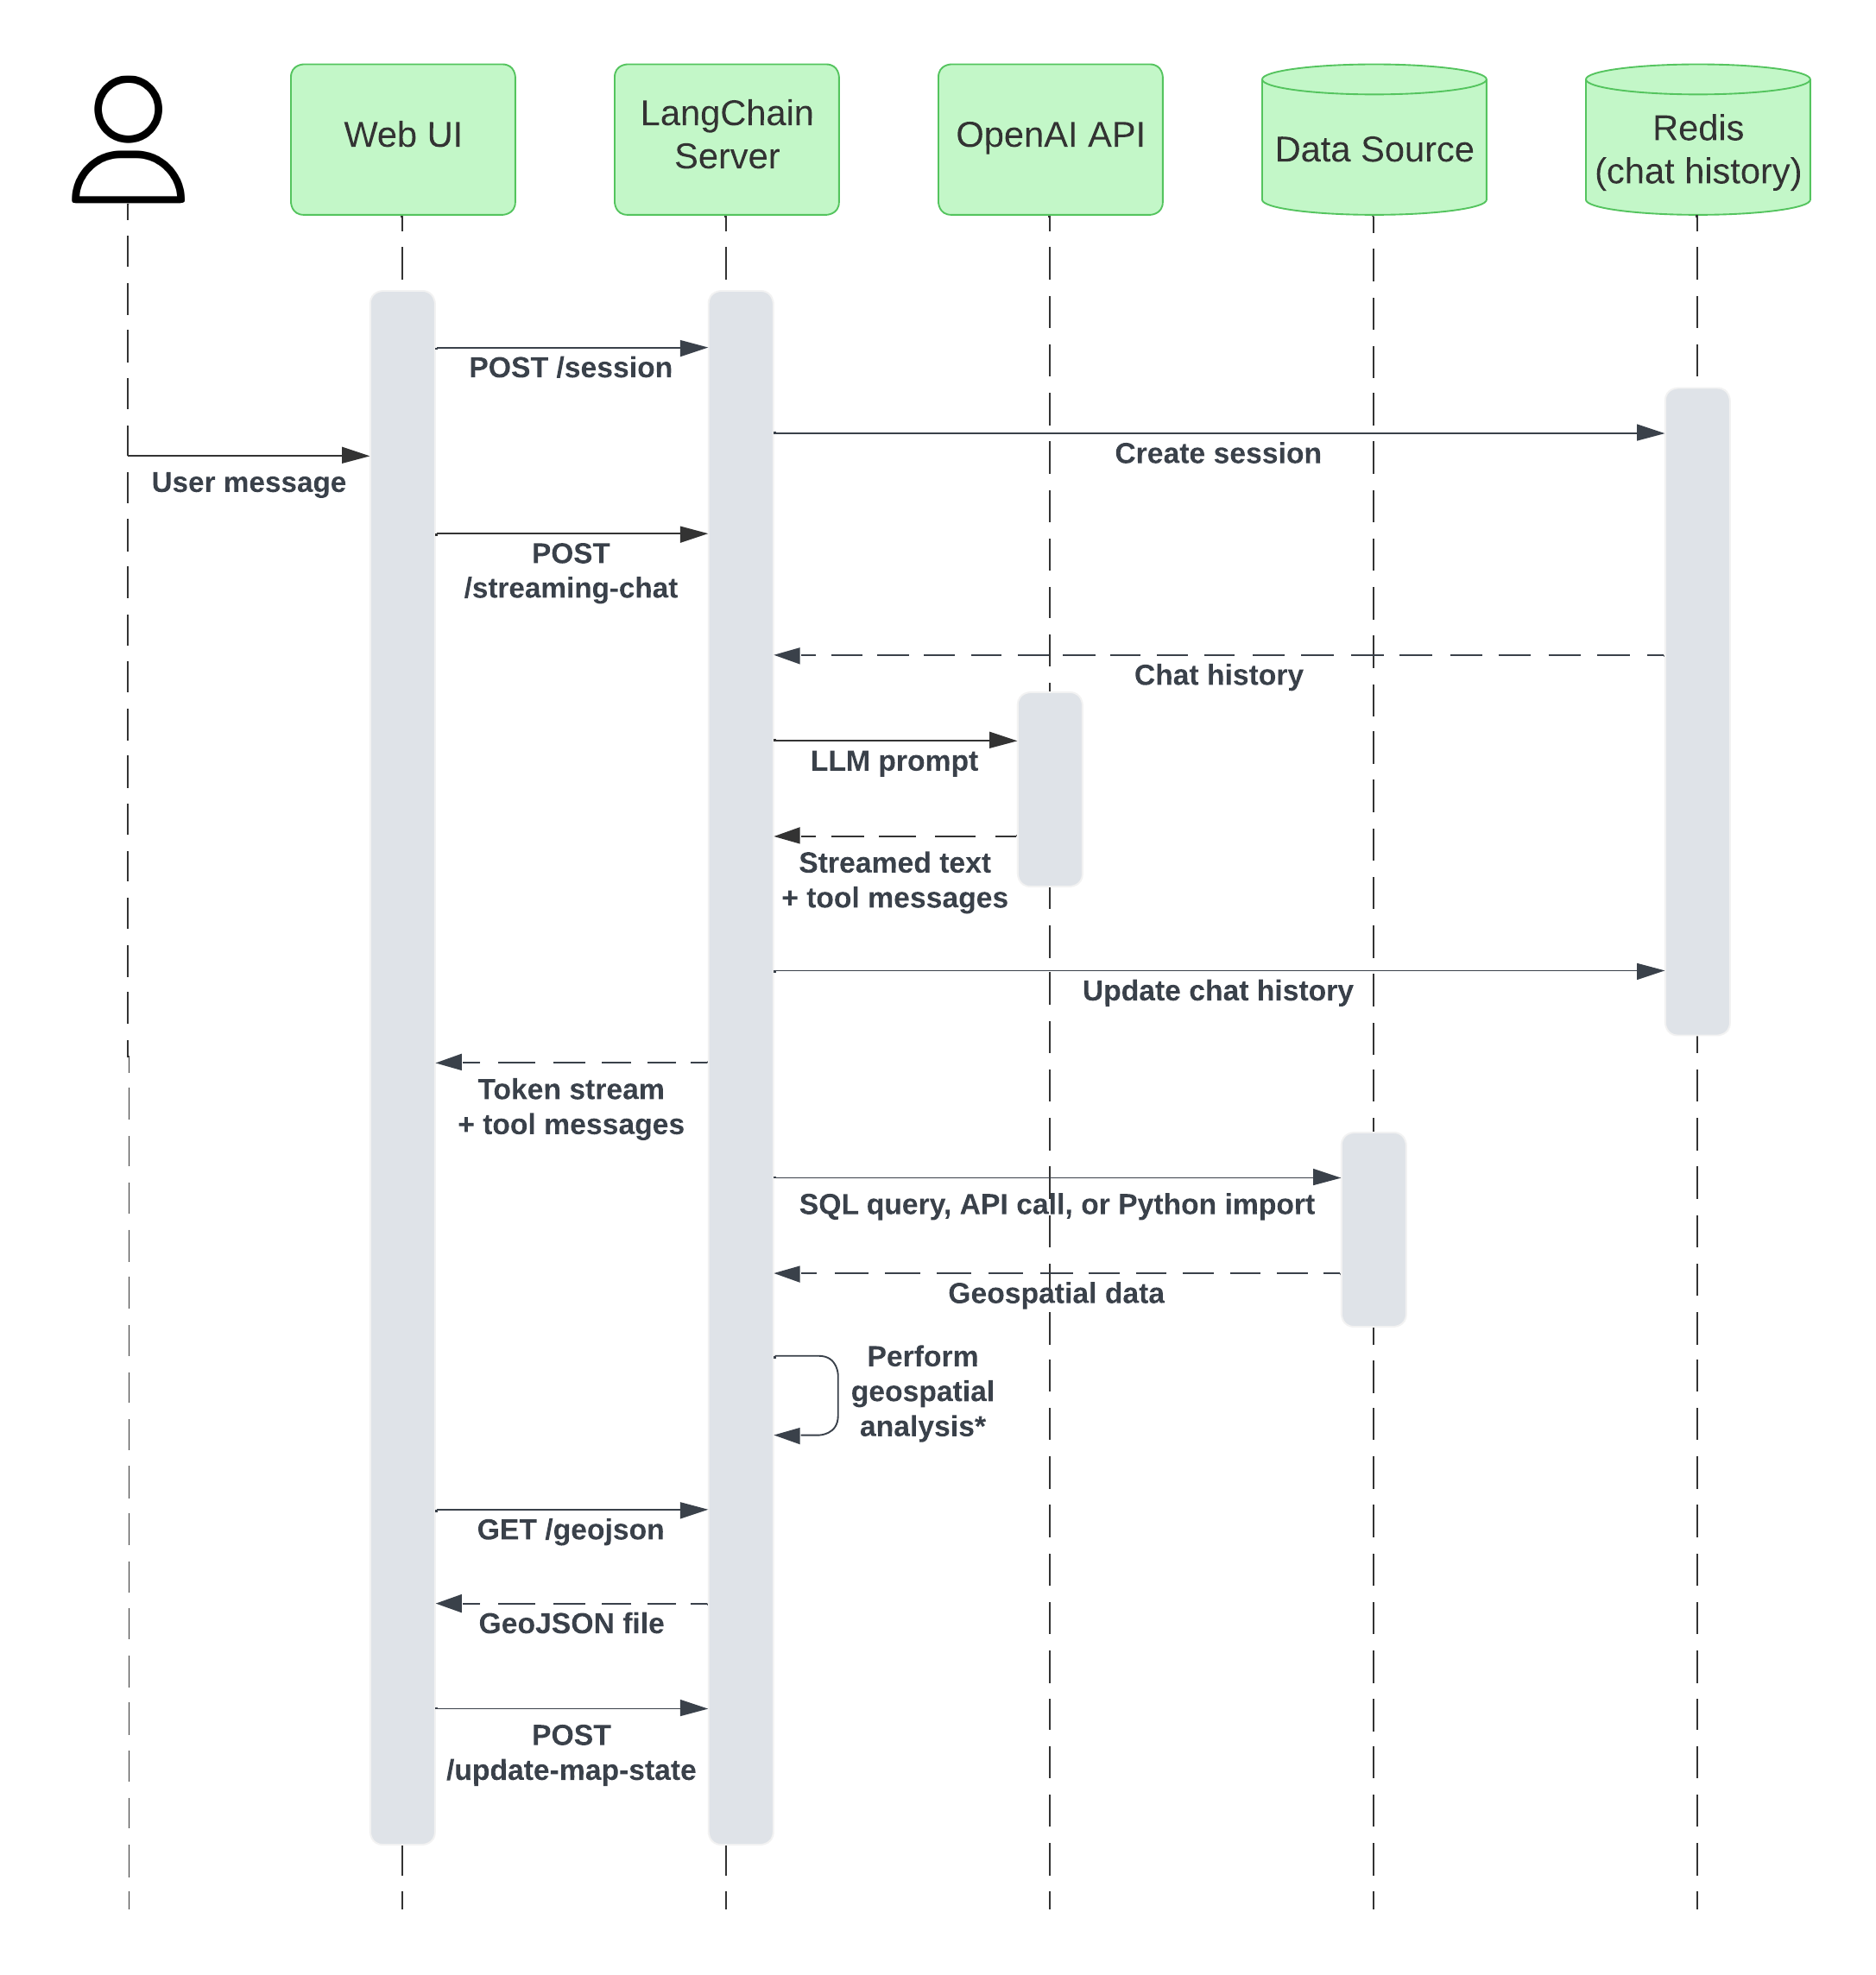
\includegraphics[width=1.2\textwidth]{Sequence diagram.png}}
    \caption{Sequence diagram showing the information flow as the user loads and sends a message to GeoGPT}
    \label{fig:sequence-diagram}
\end{figure}


\subsection{Redis for Conversations}

Redis \citep{sanfilippoRedisRealtimeData2009} is a fast in-memory database that is often applied as a caching database that sits on top of some persistent database. It can also be used for vector-based storage and as a simple NoSQL database. The latter option is the way it is used in GeoGPT's architecture, and its only purpose is to store conversations. Whenever a user starts a conversation with GeoGPT an object with a unique session ID is stored to the Redis database. This object holds an array that represents the conversation. This array is written to every time either the human or GeoGPT produces a message.

Storing messages --- either in memory as a simple array or in a database like Redis --- is crucial to enable multi-message conversations. In order for a \gls{acr:llm} to act as a conversational agent, some sort of chat history needs to be prepended to the prompt. In the case of GeoGPT the entire chat history is prepended. This has the advantage of providing the \gls{acr:llm} with the complete context of the chat history, but the disadvantage of potentially bloating the context window from which it is supposed to generate tokens. Therefore, as the chat becomes longer each new token will be both more expensive and take more time to get generated. A long chat history could also make the resulting prompt exceed the token limit of the \gls{acr:llm}, or it could confuse model by providing it with messages no longer relevant to the conversation. These issue was not considered in great detail for this project, and are left for future work.

\subsection[PostGIS and OGC API Features]{PostGIS \acrshort{acr:ogc} \acrshort{acr:api} Features}

A PostgreSQL database with the PostGIS extension containing \gls{acr:osm} data was deployed using Docker. On top of this database is a RESTful geospatial feature server called \textit{pg\_featureserv} \citep{crunchydataCrunchyDataPg_featureserv2024}. The web server is realized through the \texttt{pramsey/pg\_featureserv} Docker image\footnote{\url{https://hub.docker.com/r/pramsey/pg_featureserv}}, which is simply passed a database connection string to the database one wishes to expose on the \acrshort{acr:api}. Any tables in that database which have a geometry column and a specified \gls{acr:crs} will be exposed through the web server. pg\_featuresserv allows for features like bounding box filtering, feature limiting, and \acrshort{acr:cql} filtering. These are added as query parameters to the URL of the collection items (for instance: \texttt{.../collections/\{collection\_id\}/items.json?limit=1000\&filter=name IS NOT NULL}). In the internals of pg\_featuresserv, this URL will be converted to an \acrshort{acr:sql} query that will be run against the database. Results of the query will be returned as GeoJSON. \autoref{code:cql-to-sql} shows an example of how \acrshort{acr:cql} code is converted into \acrshort{acr:sql} code:

\begin{lstlisting}[
    language=SQL,
    label=code:cql-to-sql,
    caption=Conversion from \acrshort{acr:cql} to \acrshort{acr:sql}
]
\\ CQL code passed through the `filter` query parameter
within(geom, POINT(0 0))

\\ SQL code that will be run agains the database
ST_Within("geom",'SRID=4326;POINT(0 0)'::geometry)
\end{lstlisting}

\subsection[Web UI]{Web \acrshort{acr:ui}}

The user interface is made with SolidJS. By design, it is very minimal. One of the goals of the project is to simplify the way we do \acrshort{acr:gis} analysis. One of the key design goals was therefore to make the interface as familiar to the user as possible and lowering the chance of the user doing something wrong.

\begin{figure}[h]
    \centering
    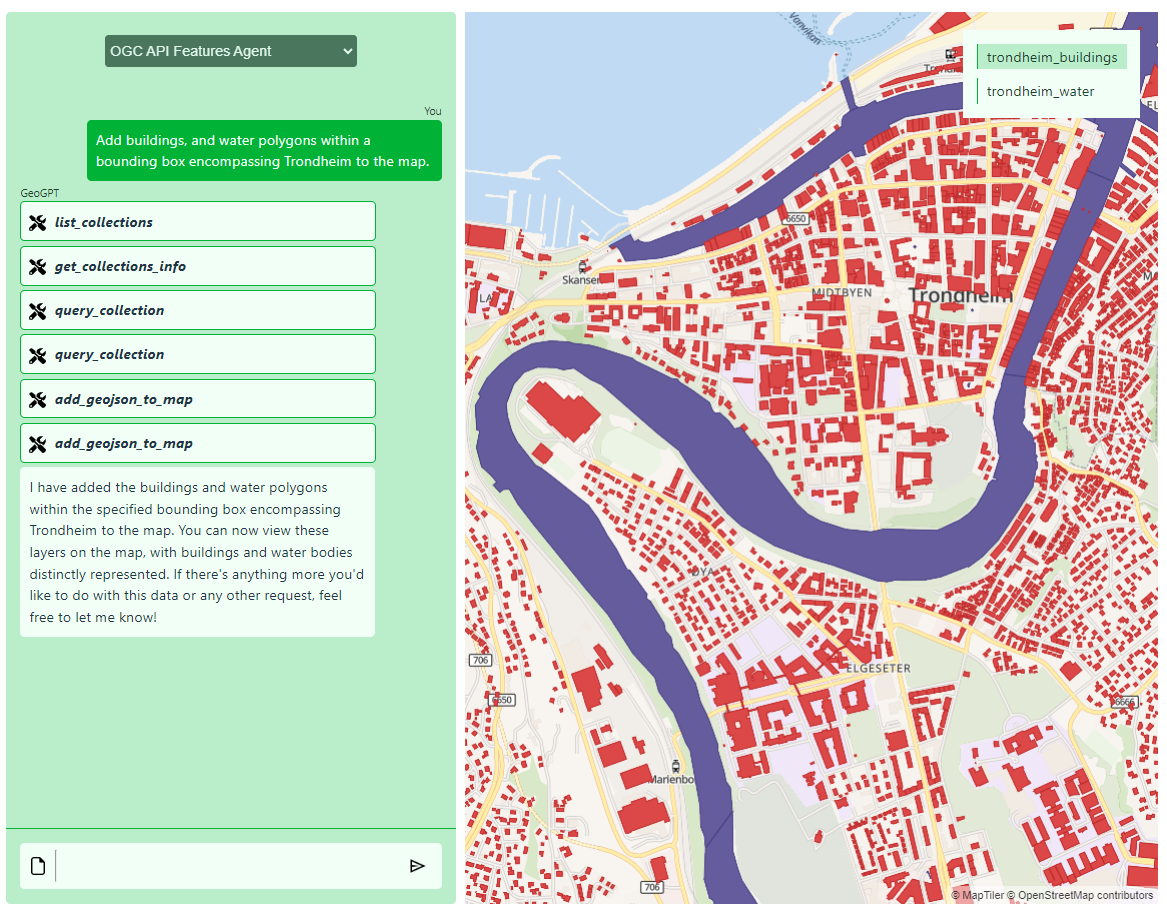
\includegraphics[width=\textwidth]{web_ui_overview_2.png}
    \caption{Web \acrshort{acr:ui}}
    \label{fig:web-ui}
\end{figure}

The chat interface was designed to imitate the interface of OpenAI's ChatGPT. Tokens and tool messages are streamed from the LangChain server, which helps the user follow the process that GeoGPT goes through when solving a problem. During this process it is possible for the user to cancel token generation if he/she sees that the system is heading off in the wrong direction. The text that is generated and streamed to the client is in Markdown format. A library called \textit{showdown}\footnote{\url{https://github.com/showdownjs/showdown}} is used to convert Markdown into \acrshort{acr:html}, ensuring that tables, code blocks, lists, and other elements are properly rendered. Next to the input field on the bottom of the chat is a file upload button. Files that are uploaded here will be added to the working directory on the LangChain server, allowing GeoGPT to perform analyses on them and optionally adding them to the map.

The map is created using MapLibre\footnote{\url{https://github.com/maplibre/maplibre-gl-js}}, an open-source fork of Mapbox which in December 2020 changed to a non-open-source software licence. A base map from \gls{acr:osm} is used, fetched through a website called MapTiler. GeoJSON files of any kind that are fetched from the server will be added to the map automatically with a random color. On the top-right of the map is an overlay listing all layers that are currently present in the map. Using the arrow keys on this list will change the z-index in the map of the selected layer.



\section{Agent Architecture}

Three different agent were implemented for GeoGPT: one agent utilizing \acrshort{acr:ogc} \acrshort{acr:api} Features, one agent which can access shapefiles using Python code, and one agent that can interact with data in an \acrshort{acr:sql} database. Common to these agents is their agentic architecture, which is described in \autoref{subsec:lg-agent-implementation}. They way that they differ is through their assigned \textit{tools}. These differences will be made apparent in \autoref{fig:tool-agent-graph}. Other slight differences are seen in the way that they are prompted. The prompting strategy used in GeoGPT and these minor differences will be discussed in \autoref{subsec:prompt-templating}.

\subsection{LangGraph Agent Implementation}
\label{subsec:lg-agent-implementation}

The agentic behaviour of GeoGPT is implemented using LangGraph, an extension to LangChain intended to make implementation of cyclic behaviour easier. \autoref{fig:tool-agent-graph} illustrates the flow between the various nodes that make up the agent. A state dictionary is passed between and updated by these nodes. Included in this state is the chat history (previous messages), the path to GeoGPT's working directory, a list of the current files in this directory, and other, less important state. The implementation is based upon a prebuilt implementation from LangGraph.\footnote{\url{https://github.com/langchain-ai/langgraph/blob/main/langgraph/prebuilt/chat_agent_executor.py}}

The \textit{\_\_start\_\_} node serves as the entry point of the agent. At this point, only one message is present in the state, namely the initial message from the user. The \textit{\_\_start\_\_} node points to the \textit{agent} node, where a response to the user is generated by an \acrshort{acr:llm}. This response could contain a textual response, or it could contain instructions to execute some tool. For this reason, the current state containing both the user message and the \acrshort{acr:ai} message, is sent to the \textit{conditional} node called \textit{agent\_should\_continue}. This node simply checks if the agent outcome (the last \acrshort{acr:ai} message) includes the \enquote{tool\_calls} keyword argument. If this is the case then some tool should be executed, and we should \enquote{continue}. If not, the agent has generated a final textual response to the user.

In the \textit{action} node the values inside the \enquote{tool\_calls} object are converted into \texttt{ToolInvocation} objects that are used to invoke predefined tools. \enquote{tool\_calls} is a list of \enquote{tool\_call} objects, each of which has attributes called \textit{name} (the name of the tool) and \textit{arguments} (arguments that should be passed to the tool). These tools are then executed, possibly having side effects on the server, and the resulting output of the tools are appended as messages to the chat history. \autoref{fig:chat-trace-example} illustrates this behaviour. This way the agent can inspect the results of the code it is \enquote{executing}, as well as being notified about possible errors in the input parameters it provided. Through the cyclic behaviour of the agent graph the agent can repeatedly call tools to try and answer the request from the user. When the agent finds to reason to call any more tools it generates a textual response, making \textit{agent\_should\_continue} return \texttt{False} so that the termination node (\textit{\_\_end\_\_}) is reached.

\begin{figure}[H]
    \centering
    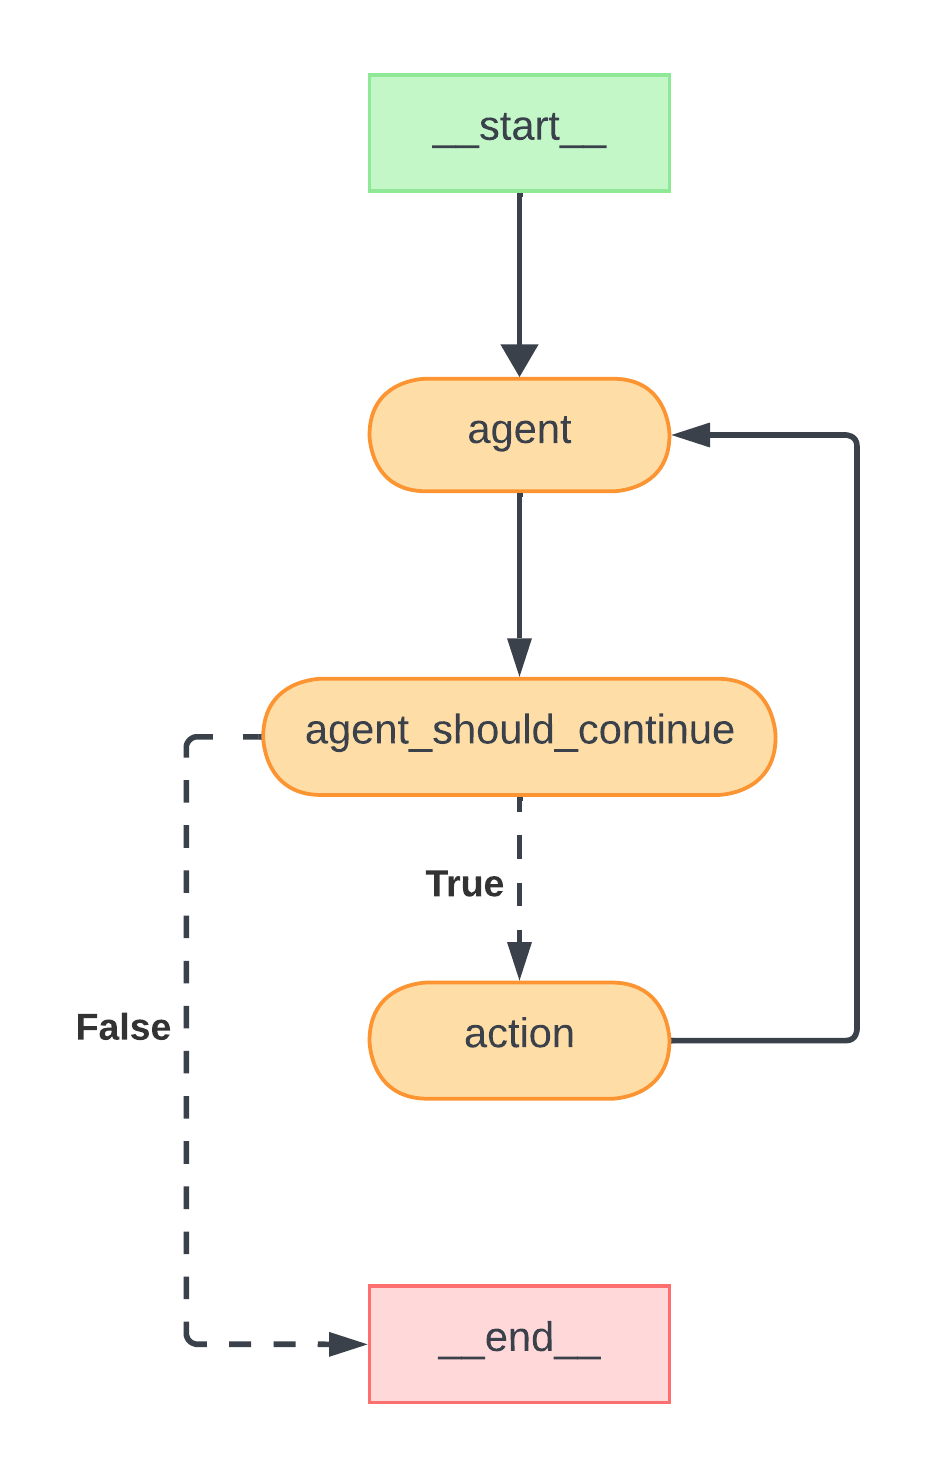
\includegraphics[width=0.6\textwidth]{agent_graph.png}
    \caption{Generic tool agent graph}
    \label{fig:tool-agent-graph}
\end{figure}

\begin{figure}
    \centering
    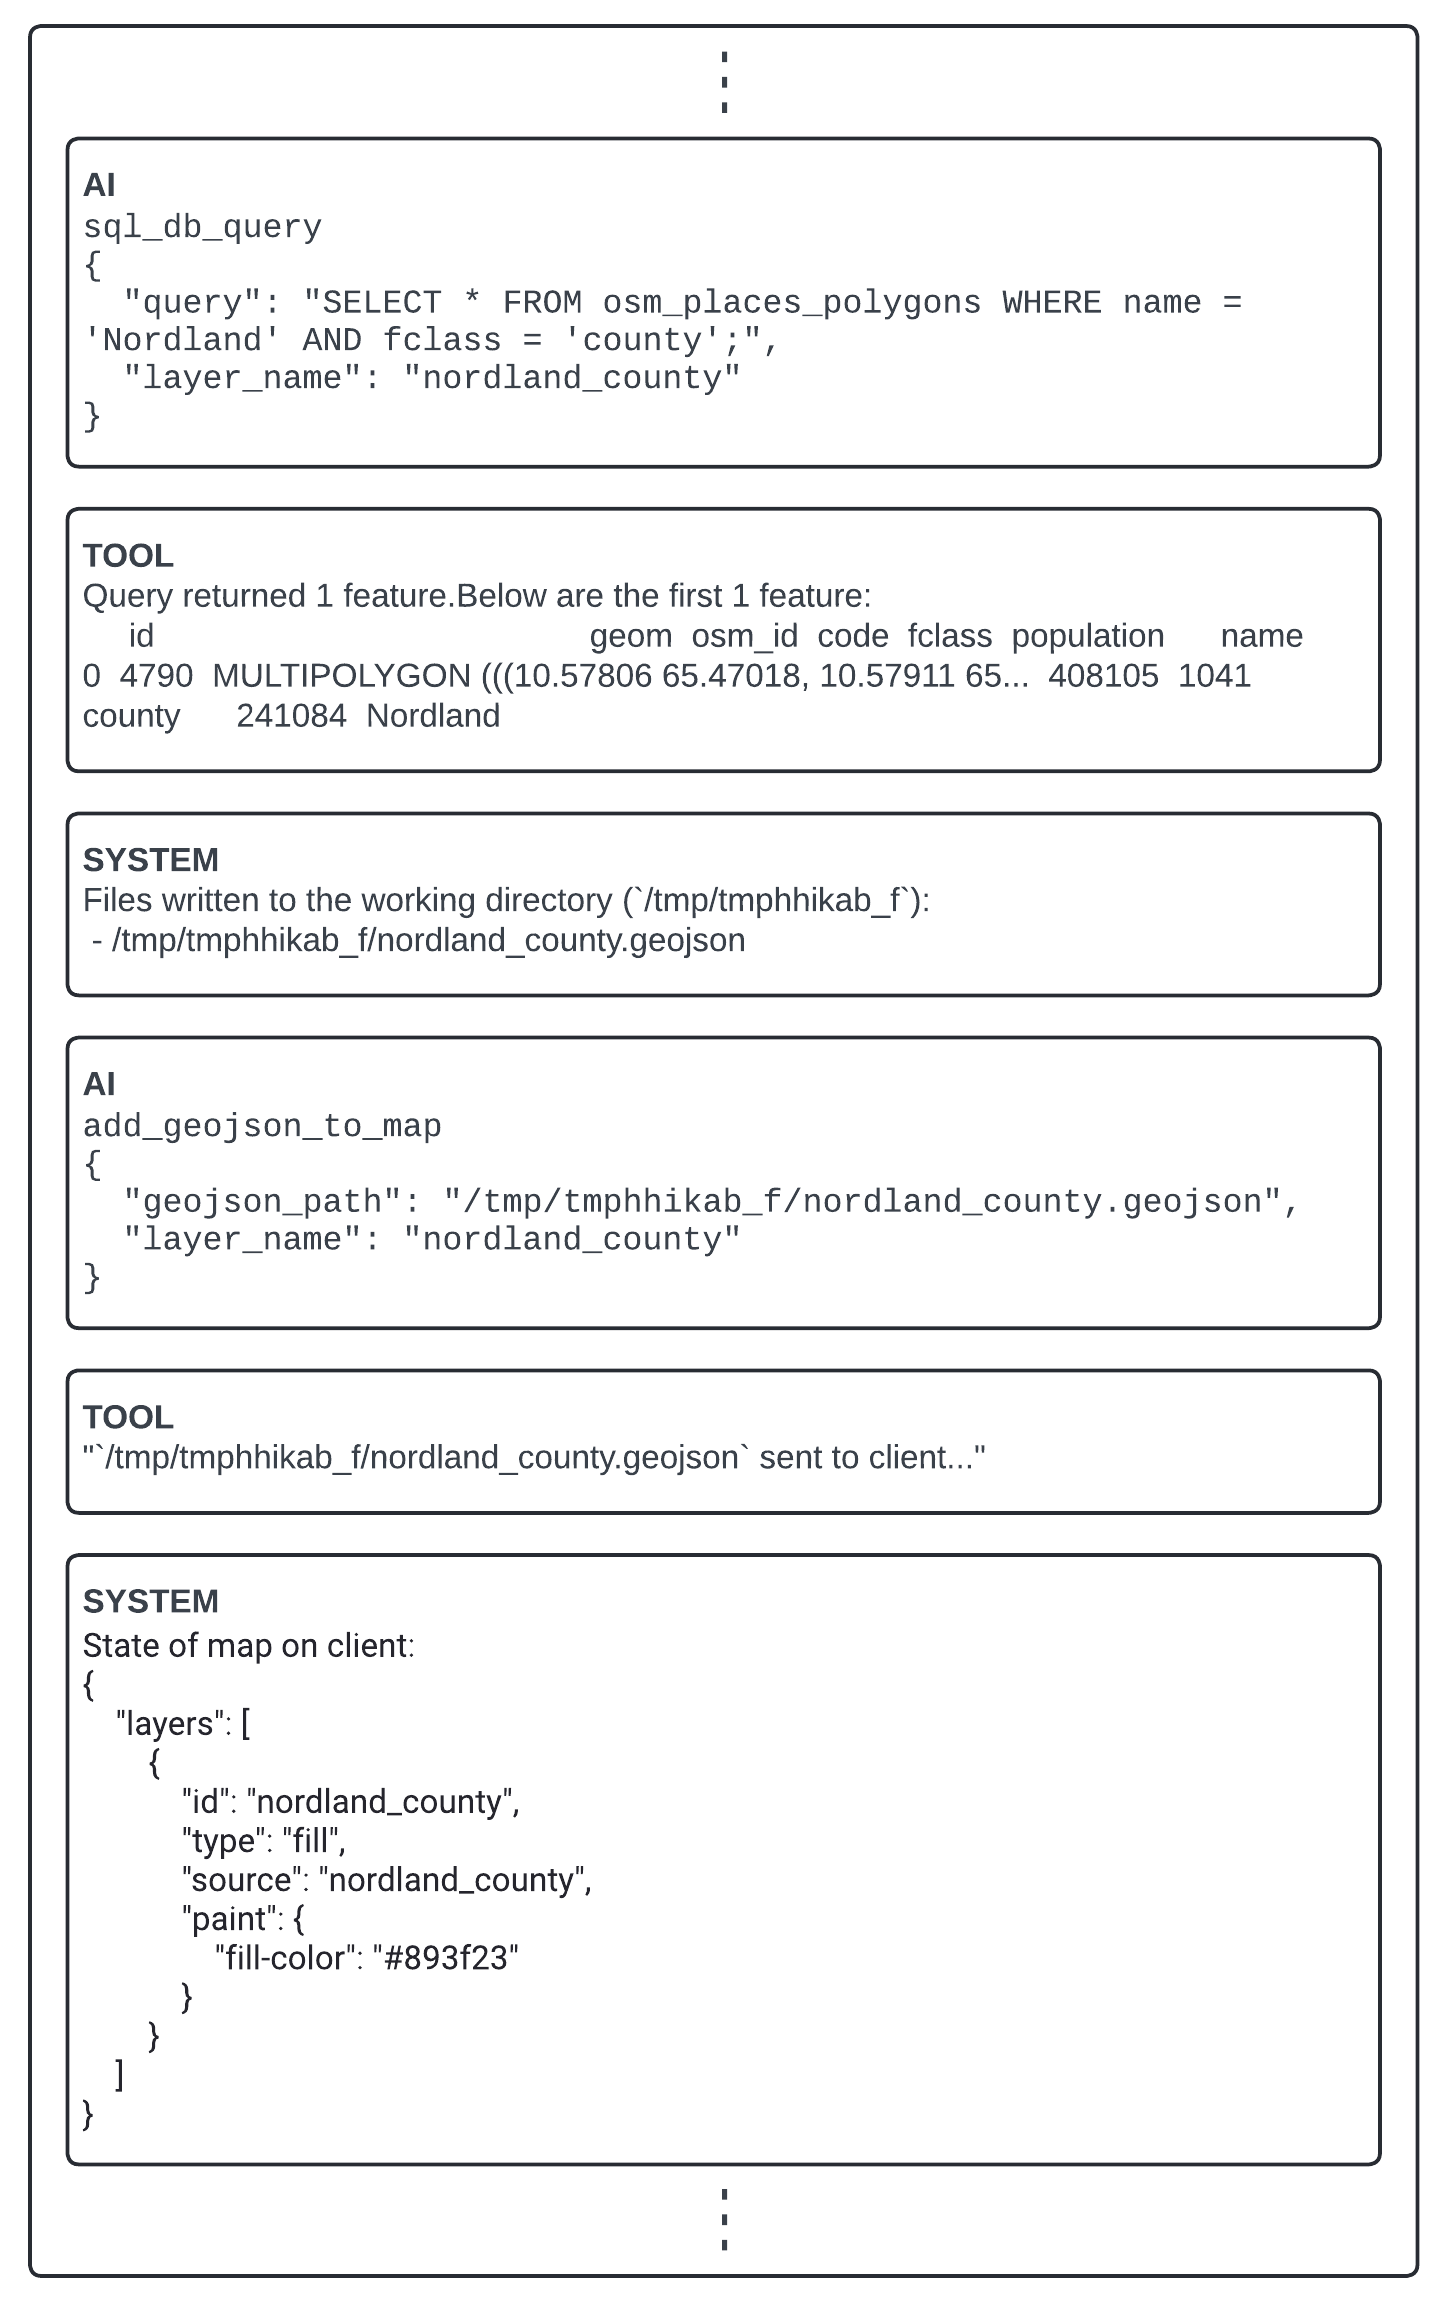
\includegraphics[width=0.9\textwidth]{query_to_client_map_chat.png}
    \caption{Example of a chat trace}
    \label{fig:chat-trace-example}
\end{figure}


\subsection{Tools}
\label{subsec:tools}

\autoref{tbl:agent-tool-overview} shows an overview of the tools that are available to each of the agents. As described in \autoref{subsec:function-calling}, these are defined by a name, an overall description of the tool's functionality, and a description of the parameters the tool expects.

The \acrshort{acr:ogc} \acrshort{acr:api} Features agent has access to a total of five tools. \textbf{\texttt{list\_collections}}, which takes no parameters, sends a \texttt{GET} request to the \texttt{/collections} endpoint and uses the response to construct a string listing the names of available collections along with their descriptions. The tool is designed to give the agent an overview of what kinds of data are available. Using the response from \texttt{list\_collections} the agent can now invoke the \textbf{\texttt{get\_collections\_info}}. This tool takes a list of collection names and returns relevant information for each of these collections. This includes the \acrshort{acr:json} response from the \enquote{landing page} of the collection, presenting details such as the collection description, spatial extent, and available attributes. In addition to this information, there is a list of common values for certain high-cardinality attributes, along with the prevalence of each value in percentages. \autoref{code:attribute-prevalences} shows an example of this. This is achieved by querying a large number of features from \texttt{/collections/\{collection\_id\}} and calculating the prevalences between them.

\begin{lstlisting}[
    caption=Prevalences of common values for the \textit{fclass} attribute in the \textit{osm\_natural\_points} collection,
    label=code:attribute-prevalences
]
Property: fclass
    tree: 71.1%
    peak: 27.2%
    beach: 0.9%
    cave_entrance: 0.5%
    spring: 0.2%
    cliff: 0.1%
    volcano: 0.0%
\end{lstlisting}

The \textbf{\texttt{query\_collection}} tool is used to retrieve features from a collection. It takes a collection name, a \acrshort{acr:cql} filter, a bounding box, and a layer name. The \acrshort{acr:cql} filter and bounding box allow for retrieval of a subset of the features of the collection being queried. Based on the parameters an URL like this is constructed:

\begin{quote}
    https://localhost:9001/collections/\{collection\_id\}/items.json?limit=10000\&filter=\{cql\_filter\}\&\{bbox\}
\end{quote}

The features retrieved from this query is saved on the working directory on the LangChain server as \enquote{\{layer\_name\}.geojson}, as a side effect of the tool. The message returned from the tool reads something like this: \enquote{Query returned 5627 features.} If the GeoJSON itself were returned as a tool message, this would quickly bloat the context window of the \acrshort{acr:llm}, and therefore it is avoided.

\begin{table}[h]
    \centering
    \caption{Overview of each agent's tools}
    \label{tbl:agent-tool-overview}
    \begin{tabularx}{0.7\textwidth}{XX}
        \toprule
        \textbf{Agent Type}                            & \textbf{Tools}                  \\
        \midrule
        \acrshort{acr:ogc} \acrshort{acr:api} Features & \texttt{list\_collections}      \\
                                                       & \texttt{get\_collections\_info} \\
                                                       & \texttt{query\_collection}      \\
                                                       & \texttt{python\_repl\_ast}      \\
                                                       & \texttt{add\_geojson\_to\_map}  \\
        \midrule
        Python                                         & \texttt{python\_repl\_ast}      \\
                                                       & \texttt{add\_geojson\_to\_map}  \\
        \midrule
        \acrshort{acr:sql}                             & \texttt{sql\_db\_list\_tables}  \\
                                                       & \texttt{sql\_db\_schema}        \\
                                                       & \texttt{sql\_db\_query}         \\
                                                       & \texttt{add\_geojson\_to\_map}  \\
        \bottomrule
    \end{tabularx}
\end{table}

Common for both the \acrshort{acr:ogc} \acrshort{acr:api} Features agent and the Python agent is the \textbf{\texttt{python\_repl\_ast}} tool. This tool accepts a string of Python code, executes said Python code, and returns whatever the code prints to the standard output in a so-called \acrfull{acr:repl}. In case the code errors, the error message is returned instead. This Python tool is the main way for these two agents perform geospatial analyses. An advantage of using \acrshortpl{acr:repl} is that the code can be executed in blocks, with variables from one block being shared with other blocks. This means that the first block may load large files into memory --- an often time-consuming operation --- while subsequent blocks can reuse this in-memory variable, even if that block should error. This allows the \acrshort{acr:llm} to quickly retry whenever the code errors or if the outcome of the initial code wasn't as expected. The \acrshort{acr:ogc} \acrshort{acr:api} Features agent will have available the files it downloaded using the \texttt{query\_collection} tool for analysis using Python, whereas the Python agent will have files corresponding to all collections available for analysis. These files are stored locally on the machine and they are added to the agent's working directory at system launch using symbolic links\footnote{\url{https://en.wikipedia.org/wiki/Symbolic_link}}. This is because a new working directory is created every time a new agent is created in order to give each agent a \enquote{clean canvas} to work from.

\textbf{\texttt{add\_geojson\_to\_map}} is the only tool that is common for all three agent types. The tool's job is to add layers to the map on the client. It takes two parameters: the name/path of a GeoJSON file stored on the LangChain server's working directory and a layer name. Invoking the tool will send a message to the client including the full path to the file on the server. The client will then make a \texttt{GET} request to the server on the \texttt{/geojson} endpoint, asking for the contents of this file to be returned so that it can be added to the map.

The \acrshort{acr:sql} agent has tools very similar to the \acrshort{acr:ogc} \acrshort{acr:api} Features agent. The \acrshort{acr:sql} agent is connected directly to the same database that the Features \acrshort{acr:api} is served on top of. \textbf{\texttt{sql\_db\_list\_tables}} is a tool that will list all database tables along with their description. \textbf{\texttt{sql\_db\_schema}} takes a list of table names and will return information about attributes, prevalence of different values in high-cardinality columns, etc., about these tables, much like \texttt{get\_collections\_info}. \textbf{\texttt{sql\_db\_query}} takes as parameter arbitrary \acrshort{acr:sql} code executes this code against the database. The tool will make sure that any query result that has a geospatial component will be stored as GeoJSON on the server. This is required to make it possible to add the geometries to the client map.


\subsection{Prompt Templating}
\label{subsec:prompt-templating}

Prompt templating is a way to produce prompts for an \acrshort{acr:llm} that follows a predefined structure. \autoref{fig:chat-template} shows an example of what the \acrshort{acr:llm} that drives GeoGPT's \acrshort{acr:sql} agent sees when the user asks which county is the largest by size.

\begin{figure}
    \centering
    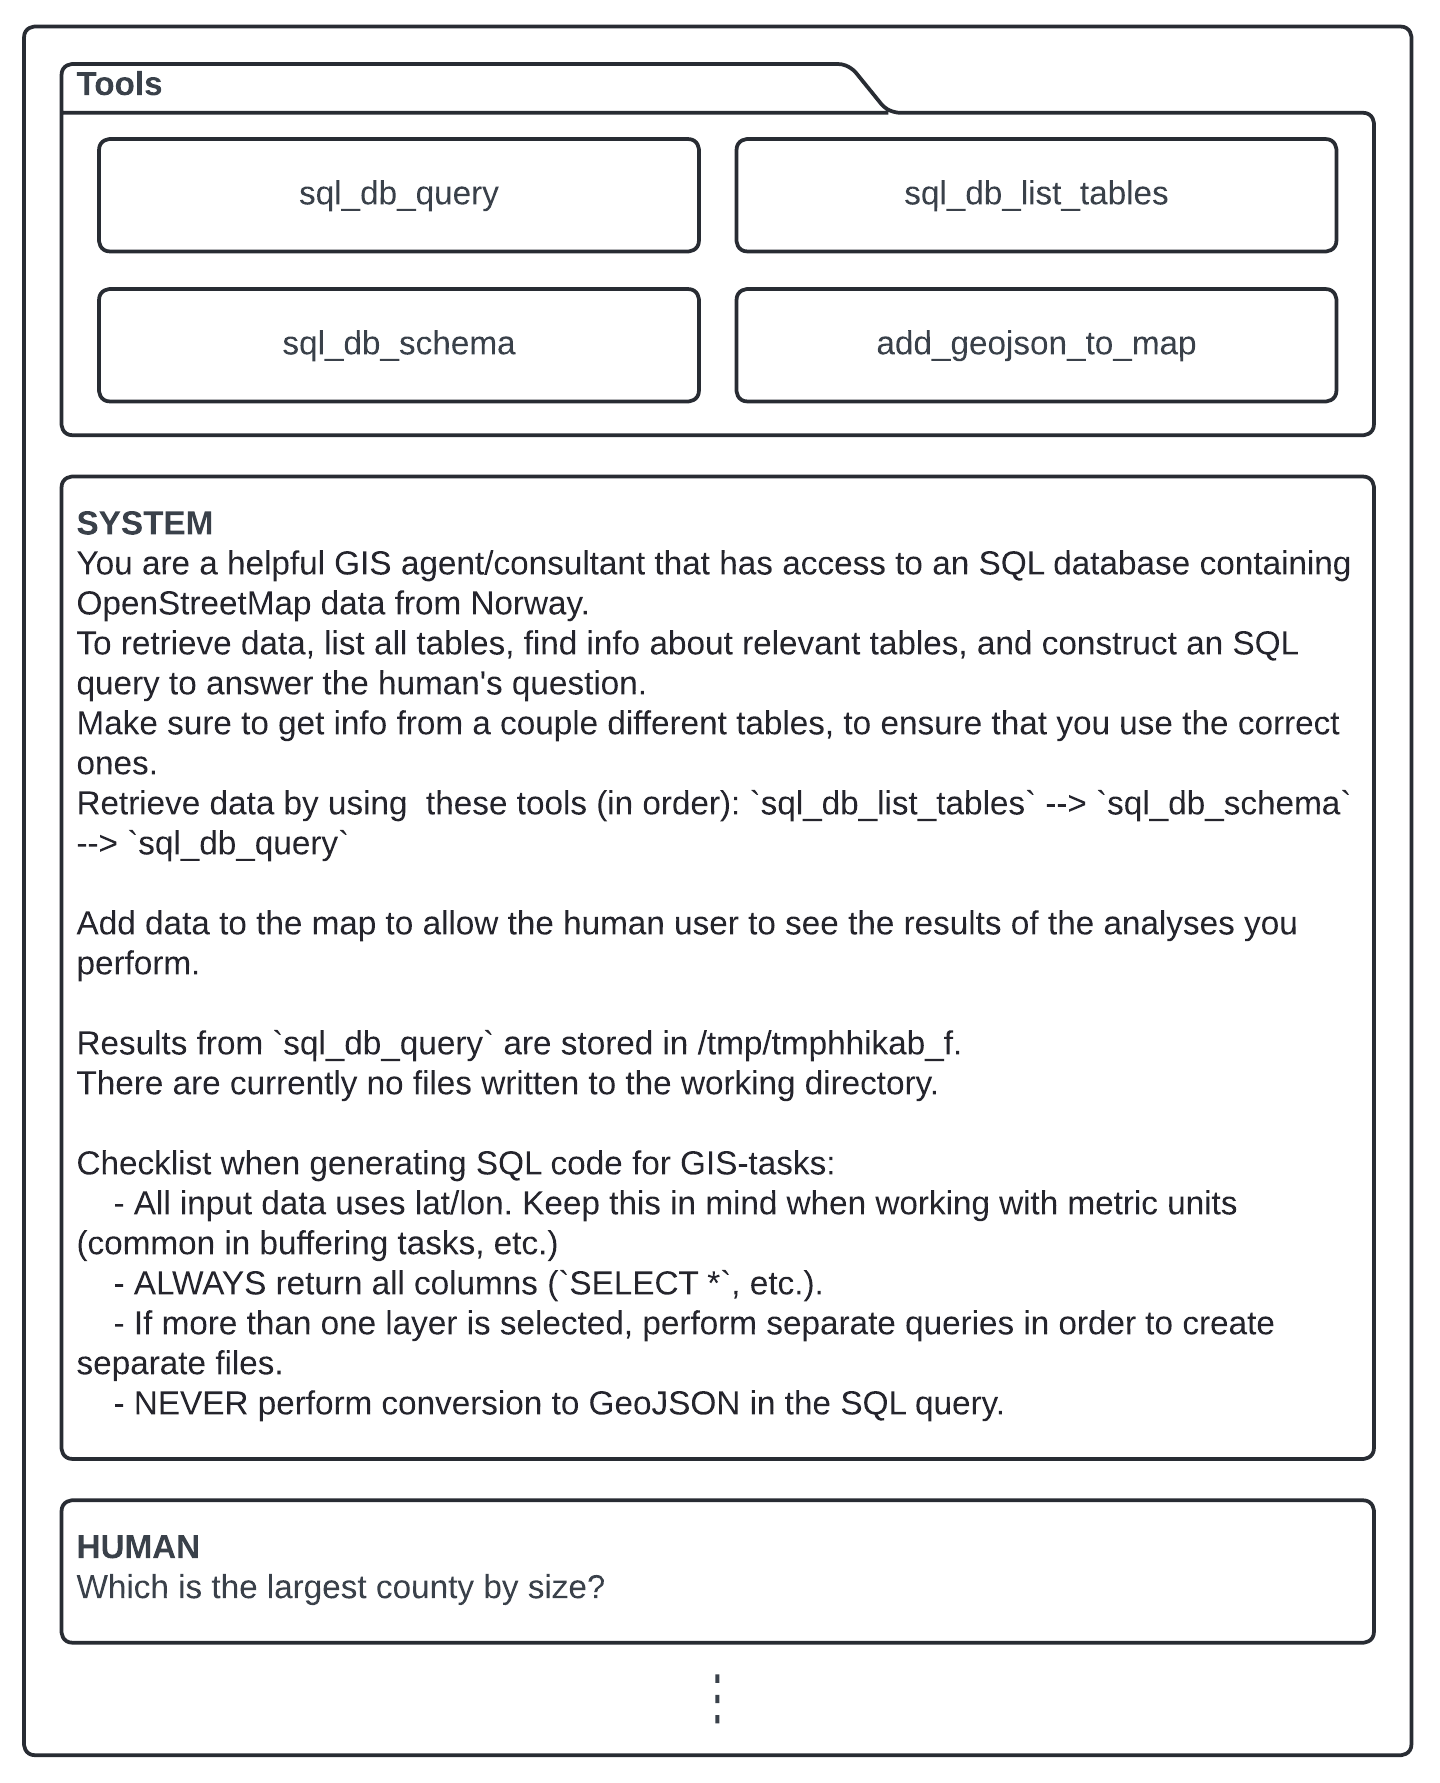
\includegraphics[width=0.9\textwidth]{template.png}
    \caption{Chat template}
    \label{fig:chat-template}
\end{figure}

The overall template consists of a collection of tools, a system message, and a chat history. Each time the \acrshort{acr:llm} in the \textit{agent} node (see \autoref{fig:tool-agent-graph}) is called this entire template is passed to it. \acrshortpl{acr:llm} have no inherent memory, so in order to have a chat conversation the entire chat history is passed with the prompt.\footnote{Several strategies have been developed by researchers to avoid having to pass the entire chat history to the \acrshort{acr:llm} each time, as this eventually will bloat the context window which could make generation slower and worse in quality. Strategies include picking only the $n$ last messages in the chat history, passing a summary of the chat instead of entire messages, or utilizing knowledge graphs.}

The system message has a structure on its own. The first half of the system message in \autoref{fig:chat-template} is intended to give the \acrshort{acr:llm} contextual awareness and hinting to how it should work towards solving tasks. We start by telling it that is \enquote{helpful \acrshort{acr:gis} agent/consultant that has access to an \acrshort{acr:sql} database containing \acrlong{acr:osm} data}. This is a common way of giving \acrshortpl{acr:llm} a persona that it can adopt, and results in responses as can be seen in \autoref{fig:effect-of-system-message}.  Continuing, we give it some information of how to string tool calls together to solve a tasks. We tell it to first list available tables, then look up schemas of relevant tables, then using the information gathered to construct an \acrshort{acr:sql} query to answer the user's request. We also remind it that it has to add the result of the analyses to the map itself (using the \texttt{add\_geojson\_to\_map} tool).

\begin{figure}[H]
    \centering
    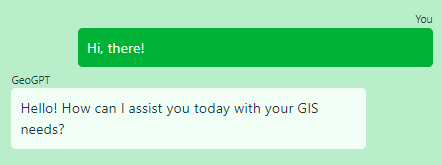
\includegraphics[width=0.6\textwidth]{hi_there.png}
    \caption{Conversation showcasing the effect of giving an \acrshort{acr:llm} a persona through the system message}
    \label{fig:effect-of-system-message}
\end{figure}

The next part of the system message concerns the working directory that GeoGPT has to work with. First, we tell it what the path to the working is. This is especially important for the \acrshort{acr:ogc} \acrshort{acr:api} Features agent and the Python agent, as they need to manually read and write to the correct path. \autoref{code:python-oslo-water-diff} shows the importance of reminding the \acrshort{acr:llm} about the location of the working directory. Having a working directory is important to control which files the agent has available, and also to make sure it doesn't save files to the folder on the server that GeoGPT is run from, as this would bloat the actual source code. Also, having a working directory lets us list the files it has available. Currently, in \autoref{fig:chat-template}, there \enquote{are currently no files written to the working directory}, but if there were they would be listed in a bullet point list.

The final part of the system message is a checklist to remind the \acrshort{acr:llm} about common pitfalls that it might run into when generating \acrshort{acr:sql} code. A similar checklist for Python is provided for the other two agents, where we remind it that it needs to use metric \acrshortpl{acr:crs} when doing area calculations, etc.

Normally, there is only a single system message in \acrshort{acr:llm}-based agents. GeoGPT, however, features a --- to the author's knowledge --- novel usage of system messages. As can be seen in \autoref{fig:chat-trace-example}, system messages are appended mid-conversation, providing updates about state changes in the system. The first system message is added because a new file has been added to the working directory, as a result of invoking the \texttt{sql\_db\_query} tool. The system message helps GeoGPT stay up-to-date on what files it has available, and it uses this information immediately to add the only file available to the map using \texttt{add\_geojson\_to\_map}. A second system message is eventually added to tell the GeoGPT that client map has been modified. The message helps ensure GeoGPT that the invocation of \texttt{add\_geojson\_to\_map} was successful. If it wasn't, the system message would inform it about this.

\glsresetall


